%***** Preamble *****%
\documentclass[a4paper]{article}

%% Language and font encodings
\usepackage[english]{babel}
\usepackage[utf8x]{inputenc}
\usepackage[T1]{fontenc}
\usepackage{graphicx}
\usepackage[font=small,labelfont=bf]{caption}
\usepackage{environ}
\usepackage{amsmath}

%% Sets page size and margins
\usepackage[a4paper,top=3cm,bottom=2cm,left=3cm,right=3cm,marginparwidth=1.75cm]{geometry}

%% Useful packages
\usepackage{amsmath}
\usepackage{graphicx}
\usepackage[colorinlistoftodos]{todonotes}
\usepackage[colorlinks=true, allcolors=blue]{hyperref}

\usepackage{float}  % Usado para posicionar imagens
\usepackage{enumitem} % Usado para criar listas enumeradas com letras
\usepackage{subcaption} % Usado para criar múltiplas imagens, uma ao lado da outra
\usepackage{hyperref} % Usado para criar hyperlinks

\usepackage{tikz} % Usado para criar FSMs
\usetikzlibrary{automata, positioning, arrows}



\usepackage{listings}
\usepackage{color}
\usepackage{xcolor}

\definecolor{vgreen}{RGB}{104,180,104}
\definecolor{vblue}{RGB}{49,49,255}
\definecolor{vorange}{RGB}{255,143,102}

\lstdefinestyle{verilog-style}
{
    language=Verilog,
    basicstyle=\small\ttfamily,
    keywordstyle=\color{vblue},
    identifierstyle=\color{black},
    commentstyle=\color{vgreen},
    numbers=left,
    numberstyle=\tiny\color{black},
    numbersep=10pt,
    tabsize=4,
    moredelim=*[s][\colorIndex]{[}{]},
    literate=*{:}{:}1
}

\makeatletter
\newcommand*\@lbracket{[}
\newcommand*\@rbracket{]}
\newcommand*\@colon{:}
\newcommand*\colorIndex{%
    \edef\@temp{\the\lst@token}%
    \ifx\@temp\@lbracket \color{black}%
    \else\ifx\@temp\@rbracket \color{black}%
    \else\ifx\@temp\@colon \color{black}%
    \else \color{vorange}%
    \fi\fi\fi
}
\makeatother

\usepackage{trace}


\title{Curso de Verilog - Dia 5}
\author{Caio Rodrigo, Jorge Reis, Manuel Adahil}
\date{} % No Date
%%%%%%%%%%%%%%%%%%%%%%%%%%%%%%%%%%%%%%%%%%%%%%%%%%%%%%%%%%%%%%%%%
%***** Document *****%
\begin{document}
\maketitle

\section*{Introdução}
Implementar um código em Verilog em FPGA exige algumas etapas prévias:

\begin{enumerate}
	\item Configurar o projeto no Vivado para realizar a síntese e implementação para uma FPGA específica, ou seja, dessa vez a escolha da FPGA na criação do projeto é relevante;
    \item Configurar o arquivo de Constraints (.xdc) no projeto para que o sintetizador possa ligar as entradas e saídas do módulo \textbf{top} em Verilog com os pinos da FPGA;
    \item Criar um módulo \textbf{top} que faça a interface dos pinos da FPGA definidos no arquivo .xdc  com os módulos do projeto.
\end{enumerate}


Usaremos a FPGA \textbf{Artix-7 XC7A35T-1CPG236C} presente na placa Basys 3 da Digilent. Portanto, na criação do projeto na tela de \textbf{Default Part} será preciso agora definir a FPGA.

Depois é preciso importar o arquivo de \textbf{.xdc} para o projeto, isso pode ser feito pelo recurso \textbf{Add Files "+"} que foi usado para criar arquivos de design e simulação. O arquivo \textbf{.xdc} para a Basys 3 pode ser encontrado \href{https://www.xilinx.com/support/documentation/university/Vivado-Teaching/HDL-Design/2015x/Basys3/Supporting%20Material/Basys3_Master.xdc}{aqui}. 

\begin{figure}[H]
	\centering
    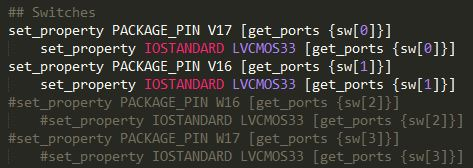
\includegraphics[width=0.5\textwidth]{images/xdc_example.jpg}
    \caption*{Exemplo de arquivo .xdc.}
\end{figure}

Repare que o arquivo .xdc vem com todas as definições comentadas. Para usar uma definição é preciso descomentá-la. Na definição é informado ao sintetizador que pino da FPGA vai ser ligado a que variável do código. Por exemplo, na imagem acima é possível ver que o pino \textbf{V17} está ligado à variável sw[0] e que o pino \textbf{V16} à variável sw[1]. Esses pinos, por sua vez, estão ligados os DIP switches mais à direita da placa.

É importante notar que as variáveis declaradas no .xdc estão na forma \textbf{sw[0]} e \textbf{sw[1]}, ou seja, elas estão declaradas na forma de um barramento \textbf{[1:0]sw}. Para mudar o nome da variável que será atrelada ao pino, é só renomear as referências à variável \textbf{sw} pelo nome desejado.

Outro ponto importante de um arquivo de constraints é que \textbf{somente poderão ser descomentadas as definições que serão utilizadas}. Caso uma definição seja descomentada não seja usada, o sintetizador irá reportar um erro.

%% newpage
\newpage

\subsection*{Exemplo}

Utilizando o .xdc da Basys 3 fornecido acima, descomente os DIP switches sw[0] e [1]. Além disso, descomente também os leds[0] e [1]. Agora vamos criar um módulo de design que será sintetizado e possuirá uma lógica combinacional.

\begin{lstlisting}[style={verilog-style}]
module TOP(
	input sw,
    output led
);

	assign led[0] = ~sw[0];
    assign led[1] = &sw;

endmodule
\end{lstlisting}

Agora sintetize e gere o bitstream para implementar o código na FPGA e verifique o funcionamento do módulo.

\section*{Prática 8 - FPGA}

\subsection*{Gates}
Utilizando os switches e os leds, reproduza o funcionamento das seguintes portas: \textbf{not},\textbf{ or}, \textbf{and}, \textbf{xor}, \textbf{nor}, \textbf{nand} e \textbf{nxor}. Cada porta, com exceção do not, possui duas entradas vindas dos switches e uma saída indo pros leds.

\subsection*{Counter}
Crie um contador de 8 bits que conte a cada um \textbf{segundo} e exiba a saída nos leds. O contador precisa ter reset e enable, ambos ativos em alto e sendo controlados por switches. 

Importante: 

\begin{itemize}
	\item É preciso reduzir a frequência do sinal de clock da FPGA no módulo para um segundo, isso pode ser feito utilizando um contado auxiliar;
    \item O contador só irá contar e resetar sincronamente quando o enable estiver ativo.

\end{itemize}

\subsection*{Display de 7 Segmentos}
Utilize os quatro displays de 7 segmentos e os switches da seguinte forma:

\begin{itemize}
	\item Cada display se associa a quatro switches, estas enviaram um valor em hexadecimal que será exibido no display;
    \item Organize os switches e displays de forma que os quatro switches mais à esquerda controlem o display mais à esquerda,
\end{itemize}

Dica: esquematize o problema e o divida em várias partes criando vários módulos, cada um resolvendo uma parte do mesmo.

\subsection*{Semáforo}
Implemente a FSM de Moore da prática do semáforo em FPGA. Utilize os switches como entradas para a FSM e o display de 7 segmentos para mostrar o estado atual e as saídas.

\end{document}